\chapter{A Cronotus projekt}

  A Cronotus projekt célja egy olyan internetes felület biztosítása, ahol az emberek könnyedén megtalálhatják a számukra legmegfelelőbb 
  sportolási lehetőségeket. Mindez egy webalkalmazás formájában valósul meg, ahová felhasználóként regisztrálva tudunk interakcióba lépni
  az elérhető sporteseményekkel, szervezőkkel.

  A rendszer igyekszik azt elérni, hogy különböző módokon hozza közelebb egymáshoz a sportolni vágyó felhasználókat. Abban az esetben, ha 
  létezik egy megfelelő sportesemény könnyedén csatlakozni lehet hozzá, ha meg nem, akkor lehetőség van egy megfelelő új esemény létrehozására.

\section{Piackutatás}
  Ahhoz, hogy jobban megérthessük a társaság hiánya okozta sportolási nehézségeket, az alábbiakban egy általunk végzett felmérést fogunk megvizsgálni.
  A felmérésben összegyűjtött adatok legfőképpen a erdélyi magyar fiataloktól származnak, korosztály szempontjából legjellemzőbben a 
  19-25 éves korig terjedő egyénekre vonatkoznak. A kutatáson 30 fő vett részt.

  \newpage

  Első sorban megbizonyosodtunk arról, hogy a fiatalok igenis érdeklődnek a sportok iránt. A felmérés kimutatta azt, hogy az egyének 90\%-a
  havonta legalább két alkalommal sportol, 36\%-uk heti szinten, míg 15\%-uk hetente többször is, ahogy ez a \ref{fig:how_much_do_people_sport}-es ábrán is látható.

  \begin{figure}[ht]
    \centering
    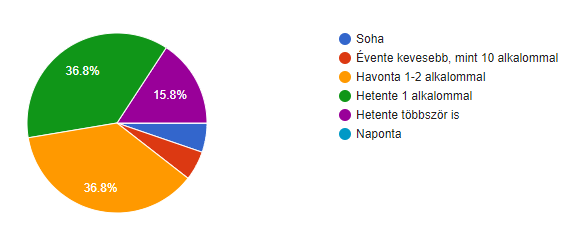
\includegraphics[width=0.8\textwidth]{./images/Screenshot 2024-04-12 162623.png}
    \caption{Mennyit sportolnak az emberek?}
    \label{fig:how_much_do_people_sport}
  \end{figure}

  A továbbiakban a felmérés azt is kimutatta, hogy sok esetben nincs elég sportolási lehetőség az egyének számára. 
  A választ adók 52\%-a azt mondta ki, hogy bár könnyen megtalálja a sporteseményeket, nincs elég lehetőség, amelyek közül válogatni lehet, míg
  az emberek 36\%-a azt mondja, hogy nehéz megtalálnia az elérhető sportolási lehetőségeket, ahogy ez látható a \ref{fig:do_you_find_options_to_sport}-es ábrán is.

  \begin{figure}[hb]
    \centering
    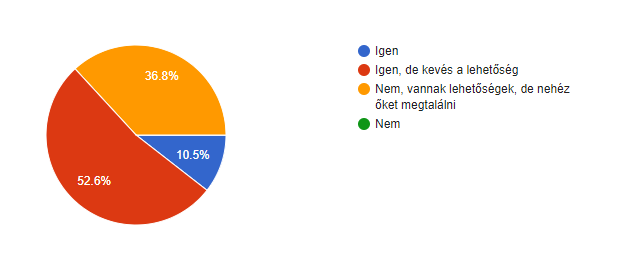
\includegraphics[width=0.8\textwidth]{./images/Screenshot 2024-04-12 165315.png}
    \caption{Könnyen talál sportolási lehetőségeket?}
    \label{fig:do_you_find_options_to_sport}
  \end{figure}

  A választ adók 100\%-ban egyetértettek abban, hogy hasznukra lenne egy olyan webalkalmazás, amely közelebb vinné őket a sportolási lehetőségekhez, 
  és elérhetővé tenné ezeket számukra, továbbá abban is teljes egyetértés volt, hogy nem ismernek más olyan alkalmazásokat,
  amely hasonló szolgáltatást nyújtana számukra.

  A felmérés arra is rámutatott, hogy az emberek azon része, akik szoktak sporteseményeket szervezni, az esetek nagyrészében 
  olyan felületet használnak, amely nem kifejezetten erre a célra készült. Legnépszerűbb megoldások közé tartozik a
  Facebook Messenger, WhatsApp, illetve más chat alapú alkalmazások használata. Ez egy egyszerű és gyors megoldás lehet, viszont 
  könnyen elveszhetnek az információk, és a szervezőknek nehéz lehet a résztvevőkkel való kommunikáció.

  A felmérésből levonható az, hogy a Cronotus projekt egy igényelt webalkalmazás, amely sok ember számára megoldást jelenthet
  a sportolással kapcsolatos nehézségekre nézve, így hozzájárulva a közösség szellemi és fizikai egészségéhez egyaránt.

\section{A Cronotus funkcionalitásai}

A Cronotus webalkalmazása a következő funkcionalításokat kínálja a felhasználó számára:

\begin{itemize}
  \item Regisztráció
  \item Bejelentkezés
  \item Felhasználói adatok listázása
  \item Felhasználói adatok szerkesztése
  \item Felhasználói profilkép és borítókép feltöltése, törlése
  \item Létrehozott sportesemények listázása
  \item Létrehozott sporteseményekre való jelentkezés, leiratkozás
  \item Saját sportesemény létrehozása előre definiált sportok alapján
  \item Saját sporteseményekhez való képek feltöltése, törlése
  \item Sportesemények törlése
\end{itemize}

\section{Szerepkörök}

  A Cronotus két fő szerepkör elkülönítésével közelíti meg a tárgyalt problémát. Az egyik az ``Organizer'', azaz szervezői, a másik pedig
  a ``Player'', avagy játékos szerepkör formájában mutatkozik meg. Egy új felhasználó regisztrálásakor automatikusan mindkét szerepkör
  jóváíródik a felhasználóhoz, így a webalkalmazás lehetőséget nyújt arra, hogy első perctől könnyedén végezhető legyen minden kívánt tevékenység.

  \subsection{A szervező}

  Ahogyan az a \ref{fig:organizer_role}-as ábrán is látható, a szervező szerepkörnek lehetősége van új sportesemények létrehozására,
  az ide tartozó információk könnyed kezelésére, valamint a résztvevőkkel való kommunikációra.
  Továbbá mindamellett, hogy eseményeket hozhat létre, lehetősége van meglévő eseményekre jelentkezni is, mint bármely más felhasználónak.

  \begin{figure}[ht]
    \centering
    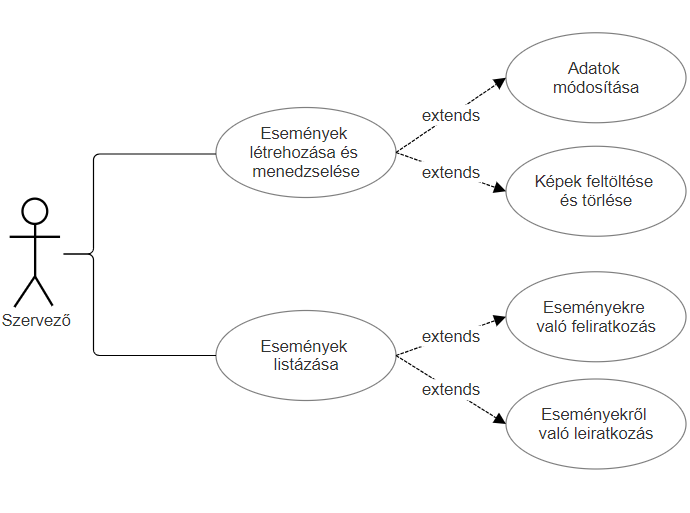
\includegraphics[width=0.8\textwidth]{./images/Screenshot 2024-04-13 021859.png}
    \caption{A szervező szerepkör}
    \label{fig:organizer_role}
  \end{figure}

  \subsection{A játékos}

  Amennyiben egy felhasználó csak arra szeretné használni a felületet, hogy sportolási lehetőségeket találjon, úgy a ``Player'' szerepkör
  lehetőségei tökéletesen elegendőek számára. A játékos felhasználók, a szervezőkhöz hasonlóan listázhatják a már létező eseményeket, 
  jelentkezhetnek ezekre, illetve figyelemmel kísérhetik az eseményekkel kapcsolatos információkat.